% \documentclass[a4paper, technote, compsoc]{IEEEtran}
\documentclass[../../thesis.tex]{subfiles}

\newcommand{\inner}[2]{\left<#1, #2\right>}
\newcommand{\alemap}{\ensuremath{\mathcal{A}}}
\newcommand{\dt}{\ensuremath{\Delta t}}
\newcommand{\pexp}{\ensuremath{\frac{2\gamma}{\left(\gamma-1\right)}}}
\newcommand{\aleX}{\ensuremath{\mathcal{X}}}
\newcommand{\Ah}[1]{\ensuremath{\vb{#1}^{n+1}_h}}
\newcommand{\Ahn}[1]{\ensuremath{\vb{#1}^{n}_h}}


\begin{document}

\section{FOM Calibration}
\label{sec:fom_calibration}
This section is devoted to present the full order model discretization details.
Certain parameters need to be defined,
along with consistency checks to validate the simulation.

Sections~\ref{sec:parameter_space_discretization} and \ref{sec:fom_response}
define the parametrization space and show some results.
In Section~\ref{sec:fom_calibration_artificial_viscosity} we show the effects of artificial viscosity,
in Section~\ref{sec:fom_calibration_bdf_convergence_rates} we explore the differences 
between BDF-1 and BDF-2 time integration schemes.

% and finally in Section~\ref{sec:fom_calibration_system_forcing} we show how
% certain combinations within the parameter space produce unfeasible solutions\footnote{
%     Due to the lack of a proper stabilization scheme. 
%     We are comfortable with this choice since it was not mandatory to
%     showcase our reduction tools.
% }, 
% and so we explain how to sample within the feasible range.

\subsection{Parameter Space and Discretization}
\label{sec:parameter_space_discretization}
To identify the reduced and collateral bases,
we randomly sample the parameter space.
We set the range for each parameter in Table~\ref{tab:parameter_range}.
The discretization parameters are given in Table~\ref{tab:discretization_parameters}.

\begin{table}[h]
    \centering
    \caption{Parameter range for random sampling.
    Note that mesh parametrizations which produce an invalid mesh
    are discarded at runtime.}
    \begin{tabular}{ccc}
    \toprule
        Variable   & Min. & Max. \\ 
        \midrule
        $a_0$      & 18      & 25      \\
        $\omega$   & 15      & 30      \\
        $\delta$   & 0.15    & 0.3     \\
        \midrule
        $x_c$      & 0.2     & 0.75    \\
        $\sigma_c$ & 0.1     & 0.2     \\
        $y_c$      & 0.25    & 1.75    \\
        \bottomrule
    \end{tabular}
    \label{tab:parameter_range}
\end{table}
% \begin{table}[h]
%     \centering
%     \caption{Piston parameter range for random sampling.}
%     \begin{tabular}{cccc}
%     \toprule
%         Variable   & Minimum & Maximum & Units 
%         \\ \midrule
%         $a_0$      & 18      & 25      & m/s \\
%         $\omega$   & 15      & 30      & 1/s \\
%         $\delta$   & 0.15    & 0.3     & [-] \\
%         $x_c$      & 0.2     & 0.75    & m   \\
%         $\sigma_c$ & 0.1     & 0.2     & m   \\
%         $y_c$      & 0.25    & 1.75    & [-] \\ 
%         \bottomrule
%     \end{tabular}
%     \label{tab:parameter_range}
% \end{table}

\begin{table}[h]
    \centering
    \caption{Space-time domain definition, and discretization parameters.}
    \begin{tabular}{cccccc}
        \toprule
        $L_0$ & $N_x$      & $T$ & $N_t$  & $\Delta x$     & $\Delta t$          \\ \midrule
        1     & 1000       & 1.0 & 500    & $\sim 10^{-3}$ & $0.5 \cdot 10^{-3}$  \\
        \bottomrule
    \end{tabular}
    \label{tab:discretization_parameters}
\end{table}
There are two relevant dimensionless groups for this problem, 
presented in Table~\ref{tab:dimensionless_groups}. 
Dimensionless groups are useful to sample the parameter space 
wisely, probing different dynamical scenarios rather
than different parametrizations which actually represent the same kind of response.
For our sampling during the offline stage (and online testing), 
we determined that taking into consideration the piston mach $u_p$ was sufficient
to collect physically distinct system responses.
\begin{table}[h]
    \centering
    \caption{Relevant dimensionless groups.
    Note that $\delta$ is a dimensionless scale parameter.}
    \begin{tabular}{cccc}
    \toprule
        Name                               & Expression                      & Min. & Max. \\ 
        \midrule
        Reduced frequency $\hat{\omega}$  & $\frac{\omega L_0}{a_0}$        & 0.6   & 1.65 \\[2mm]
        Piston mach $u_p$                 & $\frac{\delta \omega L_0}{a_0}$ & 0.1  & 0.4   \\
        \bottomrule
    \end{tabular}
    \label{tab:dimensionless_groups}
\end{table}

\subsection{FOM Response to Piston Motion}
\label{sec:fom_response}
We present the response of the system for a piston mach value $u_p = 0.37$.
The dimensionless velocity profile is shown 
in Figure~\ref{fig:fom_probes};
the mass conservation check is examined 
in Figure~\ref{fig:fom_probes_mass_conservation}.
The PDE was derived using the mass conservation principle,
but the mass conservation integral equation has not been 
used in the discretization of the weak form.
Hence it is a good independent quality check of our simulation results.

\begin{figure}[h]
    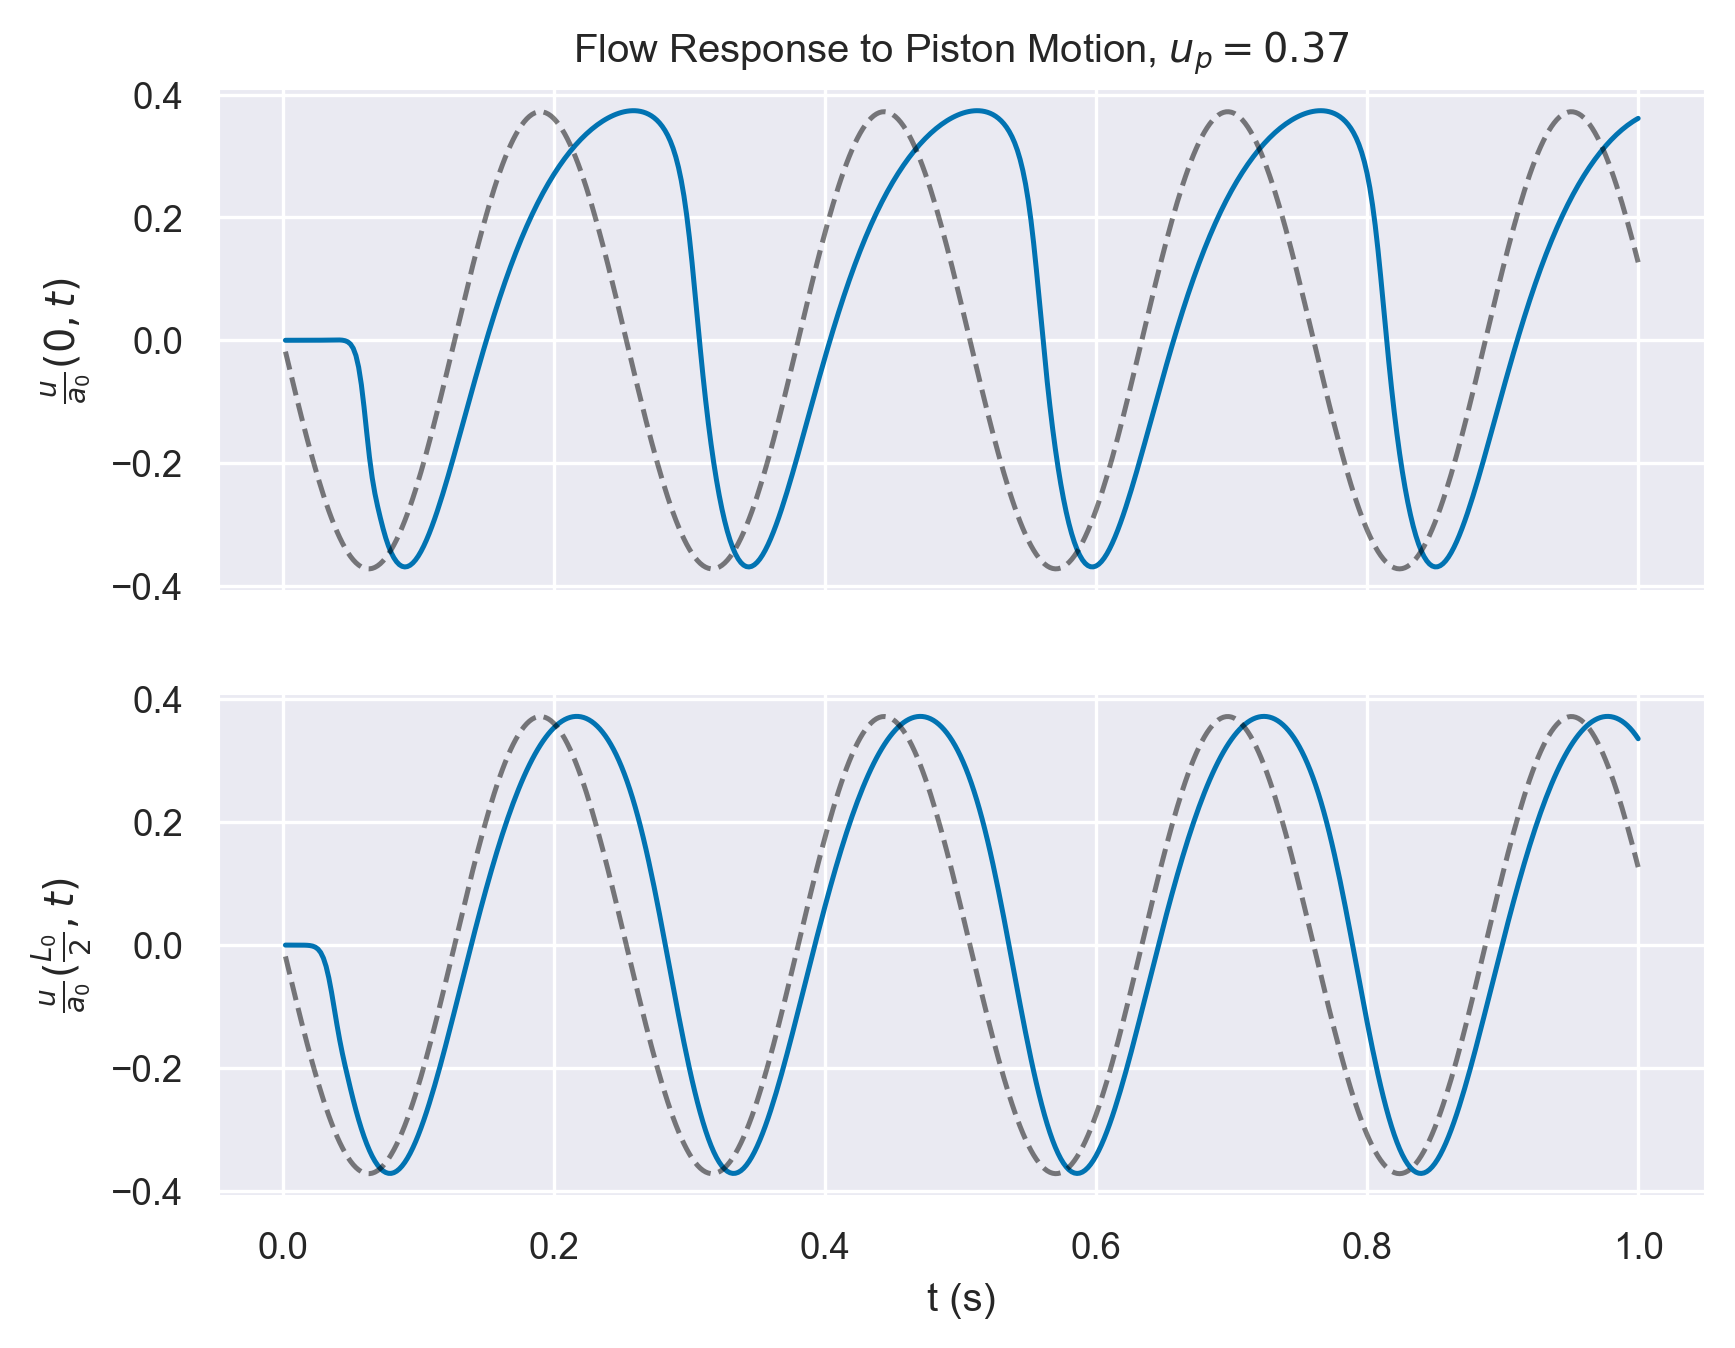
\includegraphics[width=\columnwidth]{research_project/piston/figures/fom_response/probes_online_fom_0.png}
    \caption{Flow response (blue) to piston motion (dashed).
    (Top) Piston outlet, artificial boundary condition.
    (Bottom) Piston mid-length.
    A weak shock wave is formed due to Burgers' nonlinear convection.}
    \label{fig:fom_probes}
\end{figure}

\begin{figure}[h]
    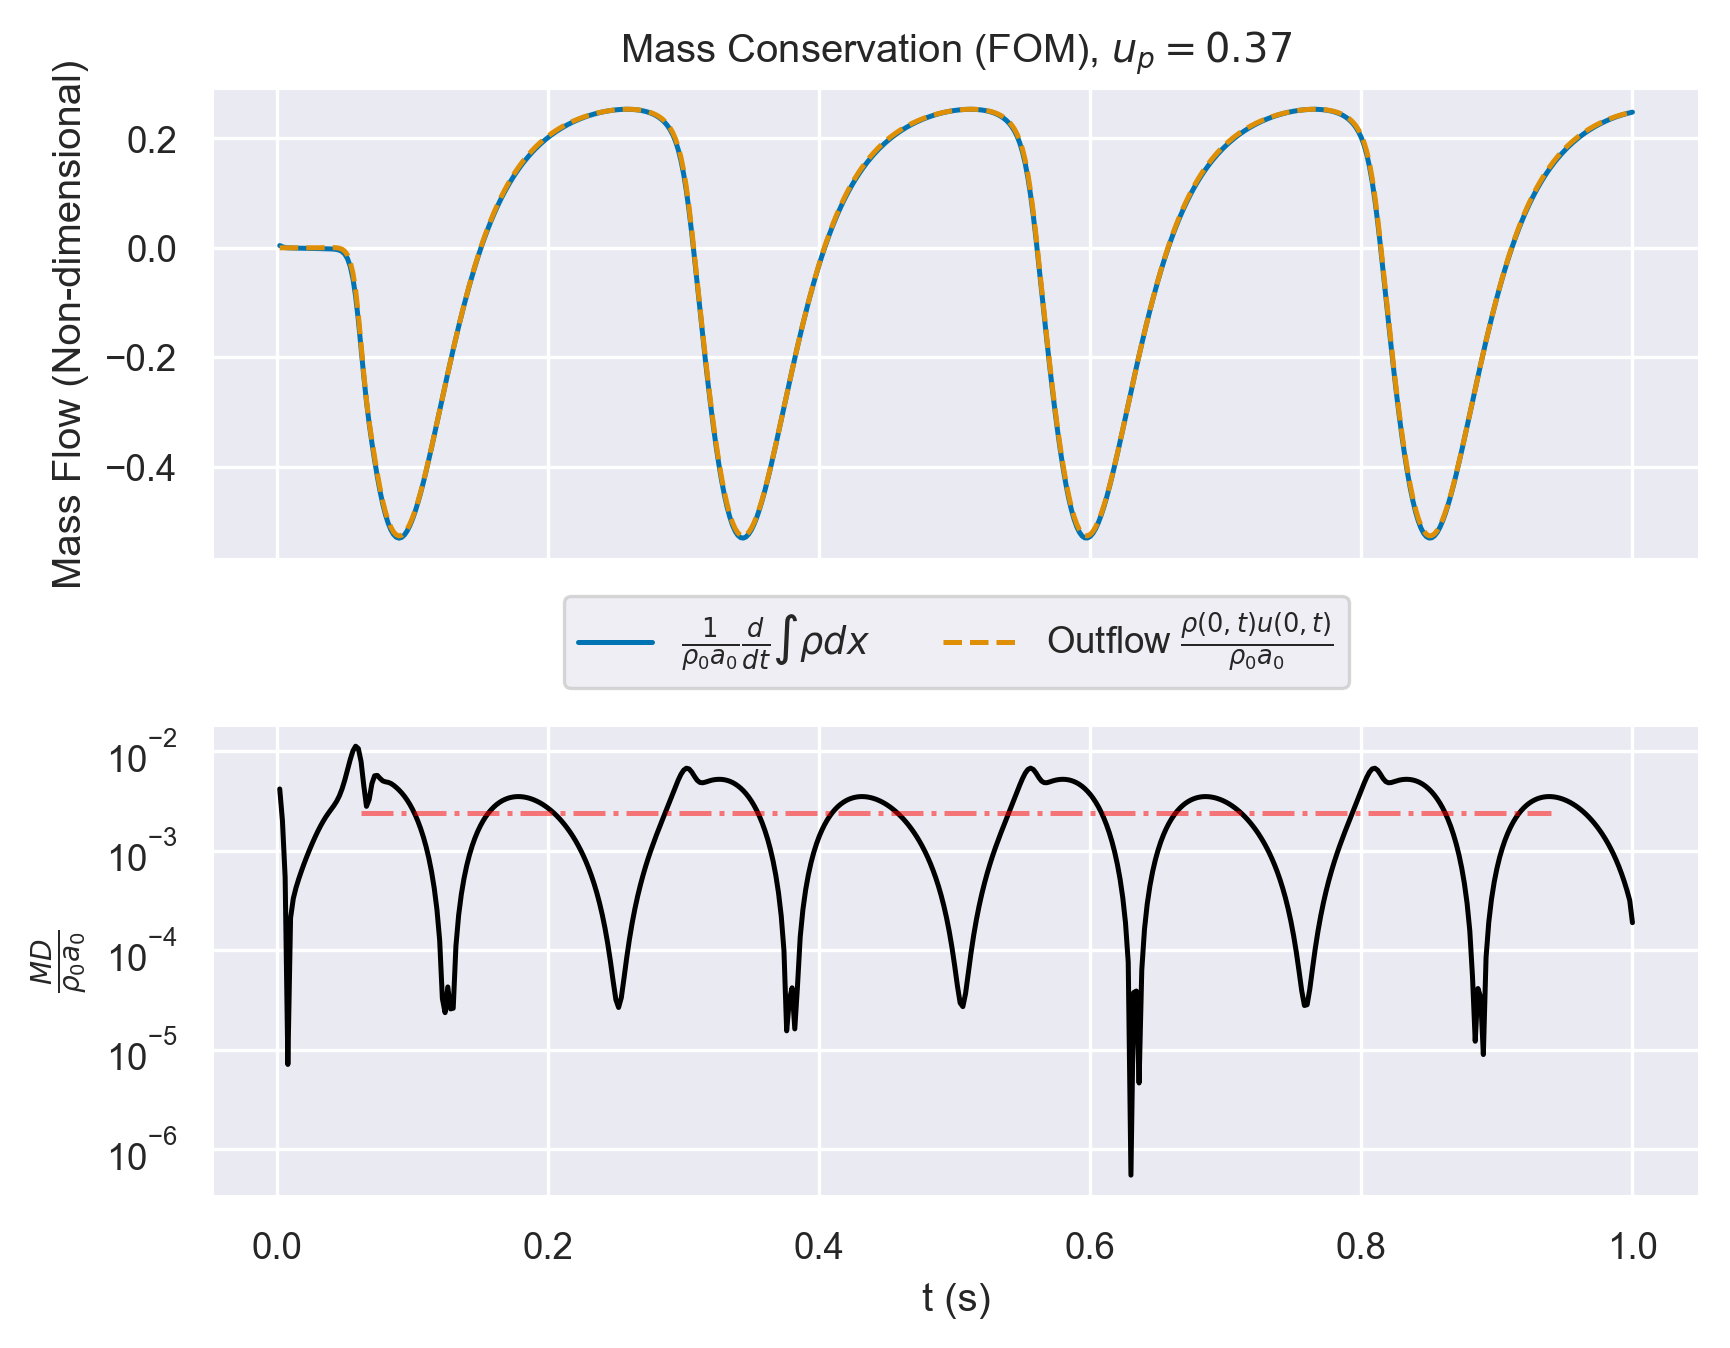
\includegraphics[width=\columnwidth]{research_project/piston/figures/fom_response/mass_conservation_online_fom_0.png}
    \caption{Mass conservation check. 
    (Top) The two resulting summands from the mass conservation integral equation:
    density integral derivative in time and outlet boundary mass flow.
    The weak shock wave is also present in the mass conservation. 
    (Bottom) Numerical value of the mass conservation principle, coined mass defect $MD$.
    The mean value (red line) is the corresponding y-axis value 
    in the convergence plot in Figure~\ref{fig:bdf_convergence_mass}.}
    \label{fig:fom_probes_mass_conservation}
\end{figure}

\subsection{Artificial Viscosity}
\label{sec:fom_calibration_artificial_viscosity}
As stated previously in the document, 
we included an artificial viscosity term in the final formulation
to go around the need for more involved\footnote{
    Note that the reduction approach used remains valid,
    since it is purely algebraic.} 
stabilization schemes.
A value needs to be choosen for the viscosity constant~$\varepsilon$.
For consistency with the PDE, 
this constant should scale with the square of the mesh size, 
\begin{equation*}
    \varepsilon \sim k \cdot (\Delta x)^2.
\end{equation*}
% A parametric sweep for different viscosity values show that this value, 
% no matter how small, was introducing measurable damping into the system.
For a mesh size of $\Delta x \sim 10^{-3}$,
the $k$-value which keeps the system stable whilst purely convective 
(at least for our simulation time scale) is
\begin{equation*}
    k = 10^{-4} \rightarrow \varepsilon \sim 10^{-10}.
\end{equation*}
In Figure~\ref{fig:artificial_viscosity_comparison} we present a comparison for these two viscosity values.
We show the motion of the fluid at the outflow and a phase plot, to ease the analysis of the correlation between the weak shock wave at the outflow and the piston motion.
The smallest viscosity value, $(10^{-10})$ leads to a \mbox{convection-like} phase plot:
the shape of the input is distorted but the maximum and mimimum values are honored, 
the same path is repeated over and over.
Instead, the solution with a higher viscosity value shows a diffusion pattern, 
reducing the extrema and changing its path on every pass.
\begin{figure}[!h]
    \centering
    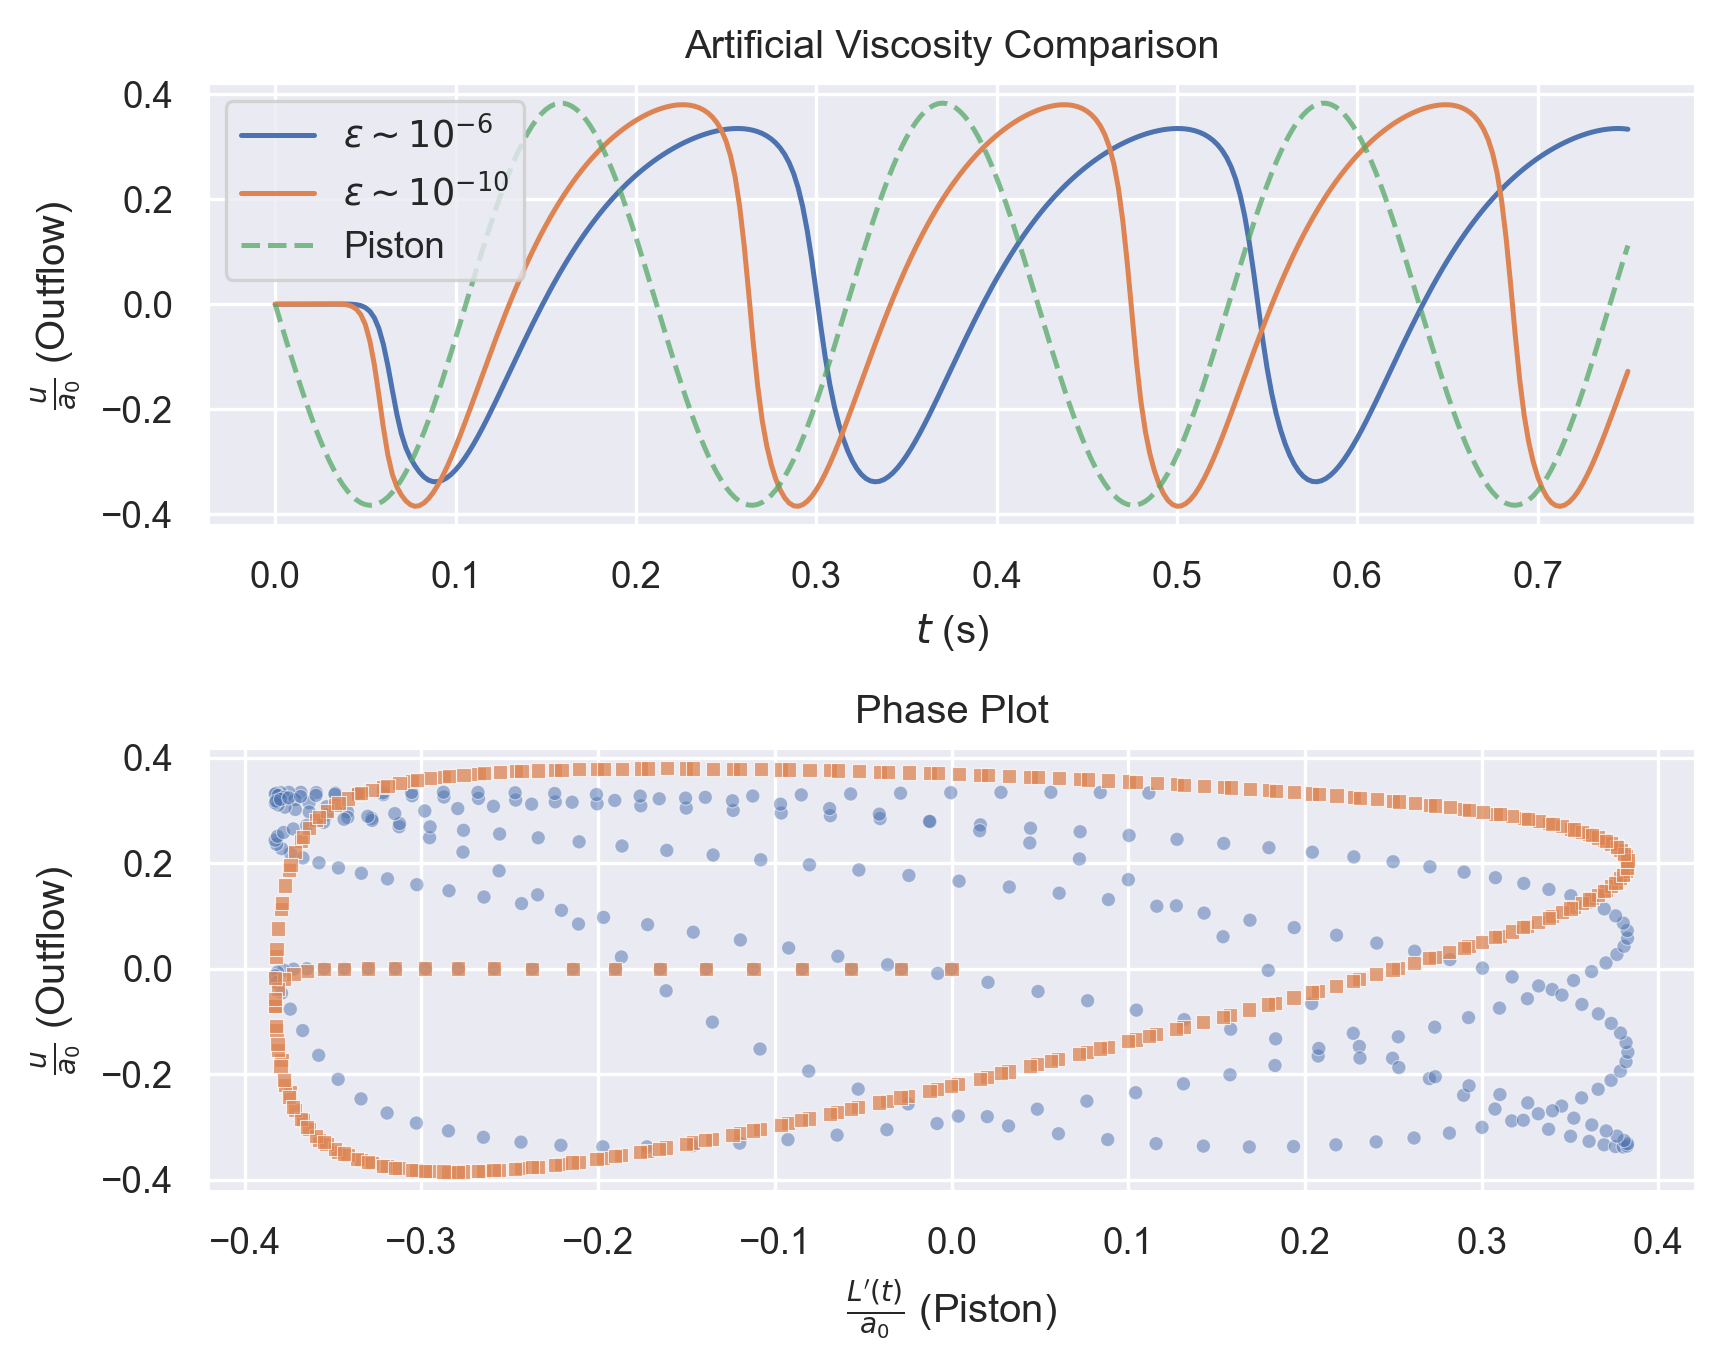
\includegraphics[width=1.0\columnwidth]{research_project/piston/figures/artificial_viscosity/artificial_viscosity_comparison.png}
    \caption{Artificial viscosity comparison.
    (Top) Outer boundary velocities for two different values of the viscosity term.
    In dashed, the piston motion, to help in the visualization of the nonlinear distortion.
    (Bottom) Phase plot between the piston motion (x-axis) and the response at the outer boundary (y-axis) for the same artificial viscosity values.
    Due to the creation of a weak shock wave, the piston motion is distorted.
    The viscosity value ($10^{-10}$) presents a stable phase plot, going over and over the same path. 
    }
    \label{fig:artificial_viscosity_comparison}
\end{figure}
% The complete reduction scheme\footnote{
%     Namely snapshot SVD compression and interpolation coefficients calculation.
% }
% seems to withstand such a small numerical viscosity term without incurring into round-off errors\footnote{If there were, we could always reduce the plain vanilla Laplace operator $\int \grad u \cdot \grad v \, \text{d}\Omega$ and scale it by $\varepsilon$ right before solving the system.}.

\newpage
\subsection{BDF Convergence Rates}
\label{sec:fom_calibration_bdf_convergence_rates}
% \mytodo{Convergence rates in space? What would be the expected rate for P1 FE?}
To check the quality of our simulations we examine 
the convergence rates for the two time-integration schemes, BDF-1 and BDF-2.
We analyze two convergence plots: the solution itself and mass preservation.

For the solution, since we do not have an analytical reference, 
we establish one numerically.
It will be the one corresponding to the solution for a small time step, 
$\Delta t = 10^{-4}$.
In Figure~\ref{fig:bdf_convergence_solutions} we present the convergence rates for the solution,
where the BDF-2 scheme ($1.98 \sim 2$) decreases twice as fast as the BDF-1 scheme ($0.95 \sim 1$).

For the mass defect, we do know it should tend to zero analytically.
In Figure~\ref{fig:bdf_convergence_mass} we give the convergence rates for the mass defect,
where the BDF-2 scheme ($2.08 \sim 2$) is seen to converge 
twice as fast as the BDF-1 scheme ($1.24 \sim 1$).
Hence, the BDF-2 scheme is correctly implemented.
\begin{figure}[h]
    \centering
    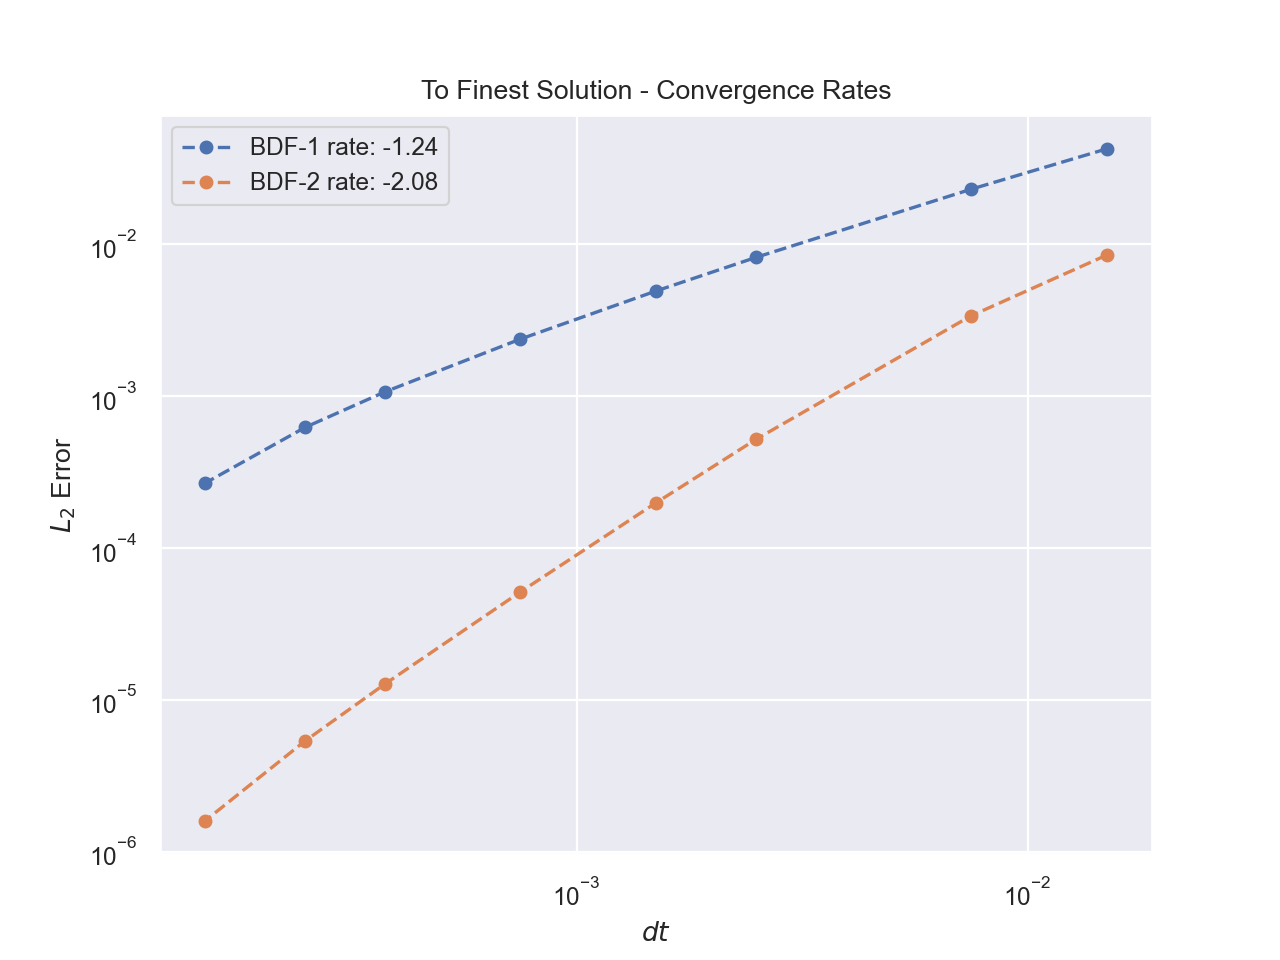
\includegraphics[width=1\columnwidth]{research_project/piston/figures/bdf_convergence/convergence_finest_solution.png}
    \caption{Convergence rates to numerical reference solution.
    The reference was obtained with a small time step, $\Delta t = 10^{-4}$.
    Both schemes decrease at their expected rates.}
    \label{fig:bdf_convergence_solutions}
\end{figure}

\begin{figure}[h]
    \centering
    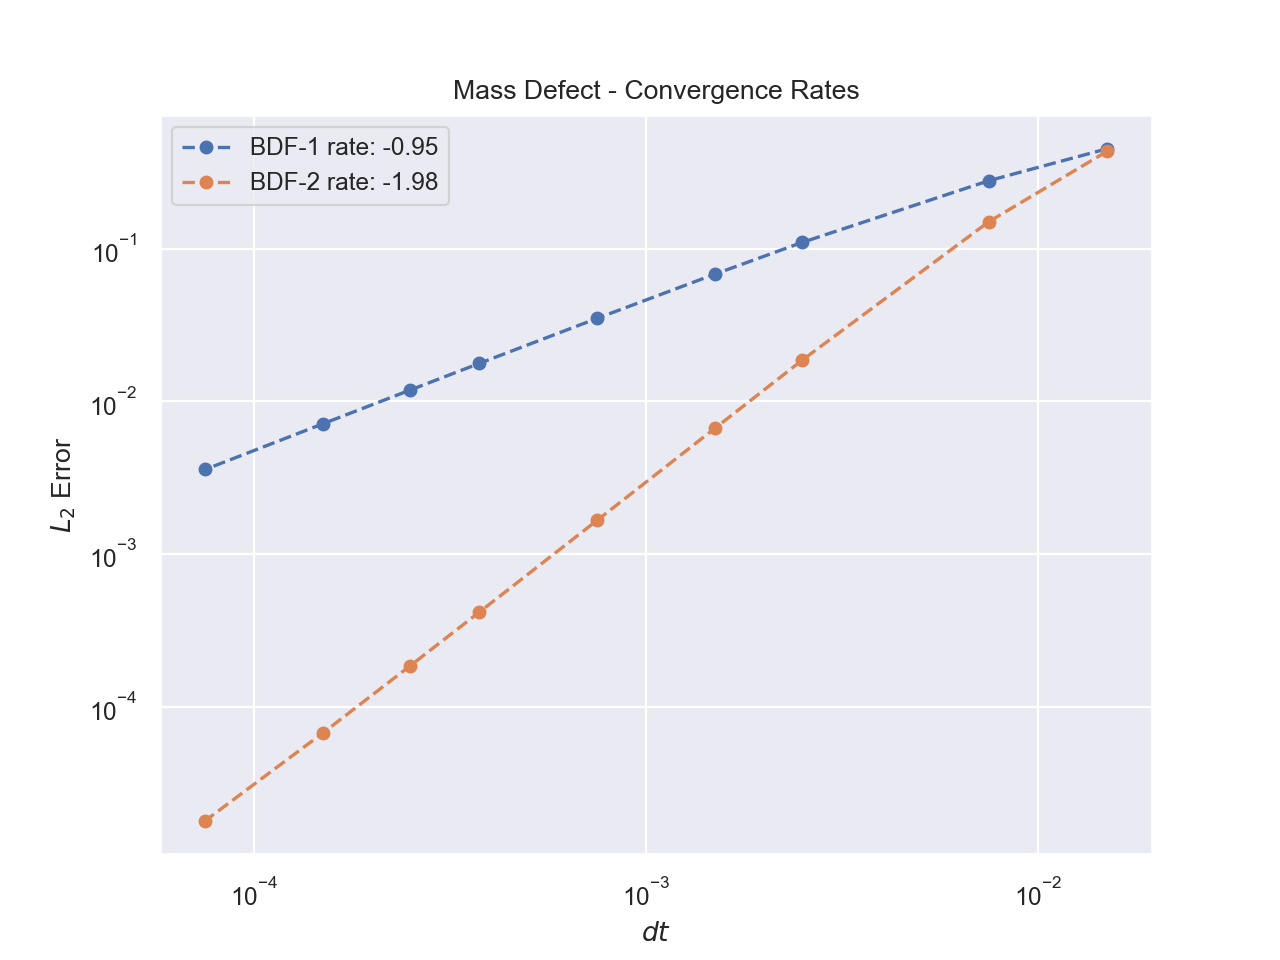
\includegraphics[width=1\columnwidth]{research_project/piston/figures/bdf_convergence/convergence_rates_mass.png}
    \caption{Convergence rates for mass defect $MD$.
    The analytical solution of this variable is zero (mass is perfectly preserved).
    Both schemes decrease at their expected rates.}
    \label{fig:bdf_convergence_mass}
\end{figure}

% \subsection{Deforming Mesh Effects}

% \subsubsection{Mesh Velocity}
% \mytodo{Show mass conservation without ALE convective term.}

\subsection{Non-Uniform Mesh Displacement}
Not all geometrical parametrizations of the mesh displacement are valid.
As shown in Table~\ref{tab:mesh_disp_params}, some parametrizations
lead to non-invertible mappings.
This takes place when the displacement is so large locally 
that the mesh nodes ordering is lost in the physical domain.
When this happens, two points in the reference domain map to the same point in the physical space.
\begin{table}[h]
    \centering
    \caption{Mesh deformation parametrizations.}
    \begin{tabular}{lccccc}
        \toprule
        {}                                      & $\delta$ & $x_c$                & $\sigma_c$           & $y_0$  & Invertible \\
        \midrule
        Figure~\ref{fig:mesh_disp_compression}  & \multirow{3}{*}{0.3}         & \multirow{3}{*}{0.5} & \multirow{3}{*}{0.1} & 0.5    & \multirow{2}{*}{Yes} \\
        Figure~\ref{fig:mesh_disp_expansion}    &          &           &                      & 0.75   & \\ 
        % \midrule[0.01mm]
        Figure~\ref{fig:mesh_disp_expansion_unfeasible} &  &           &                      & 1.75   & No \\
        \bottomrule
    \end{tabular}        
    \label{tab:mesh_disp_params}
\end{table}

The correct procedure to deal with the mesh feasibility problem 
would be to compute the Jacobian analytically
and derive from it upper and lower bounds for each parameter.
However, for such a simple domain transformation, 
we opt to check numerically at runtime if the mesh is feasible or not.
In fact, to prevent round-off errors,
we impose a lower bound on the mesh step size. 
When it is breached,
\begin{equation}
    \forall \, i \quad &\Delta x_i < 10^{-6}, 
\end{equation}
we discard that parametrization.

\begin{figure}[h]
    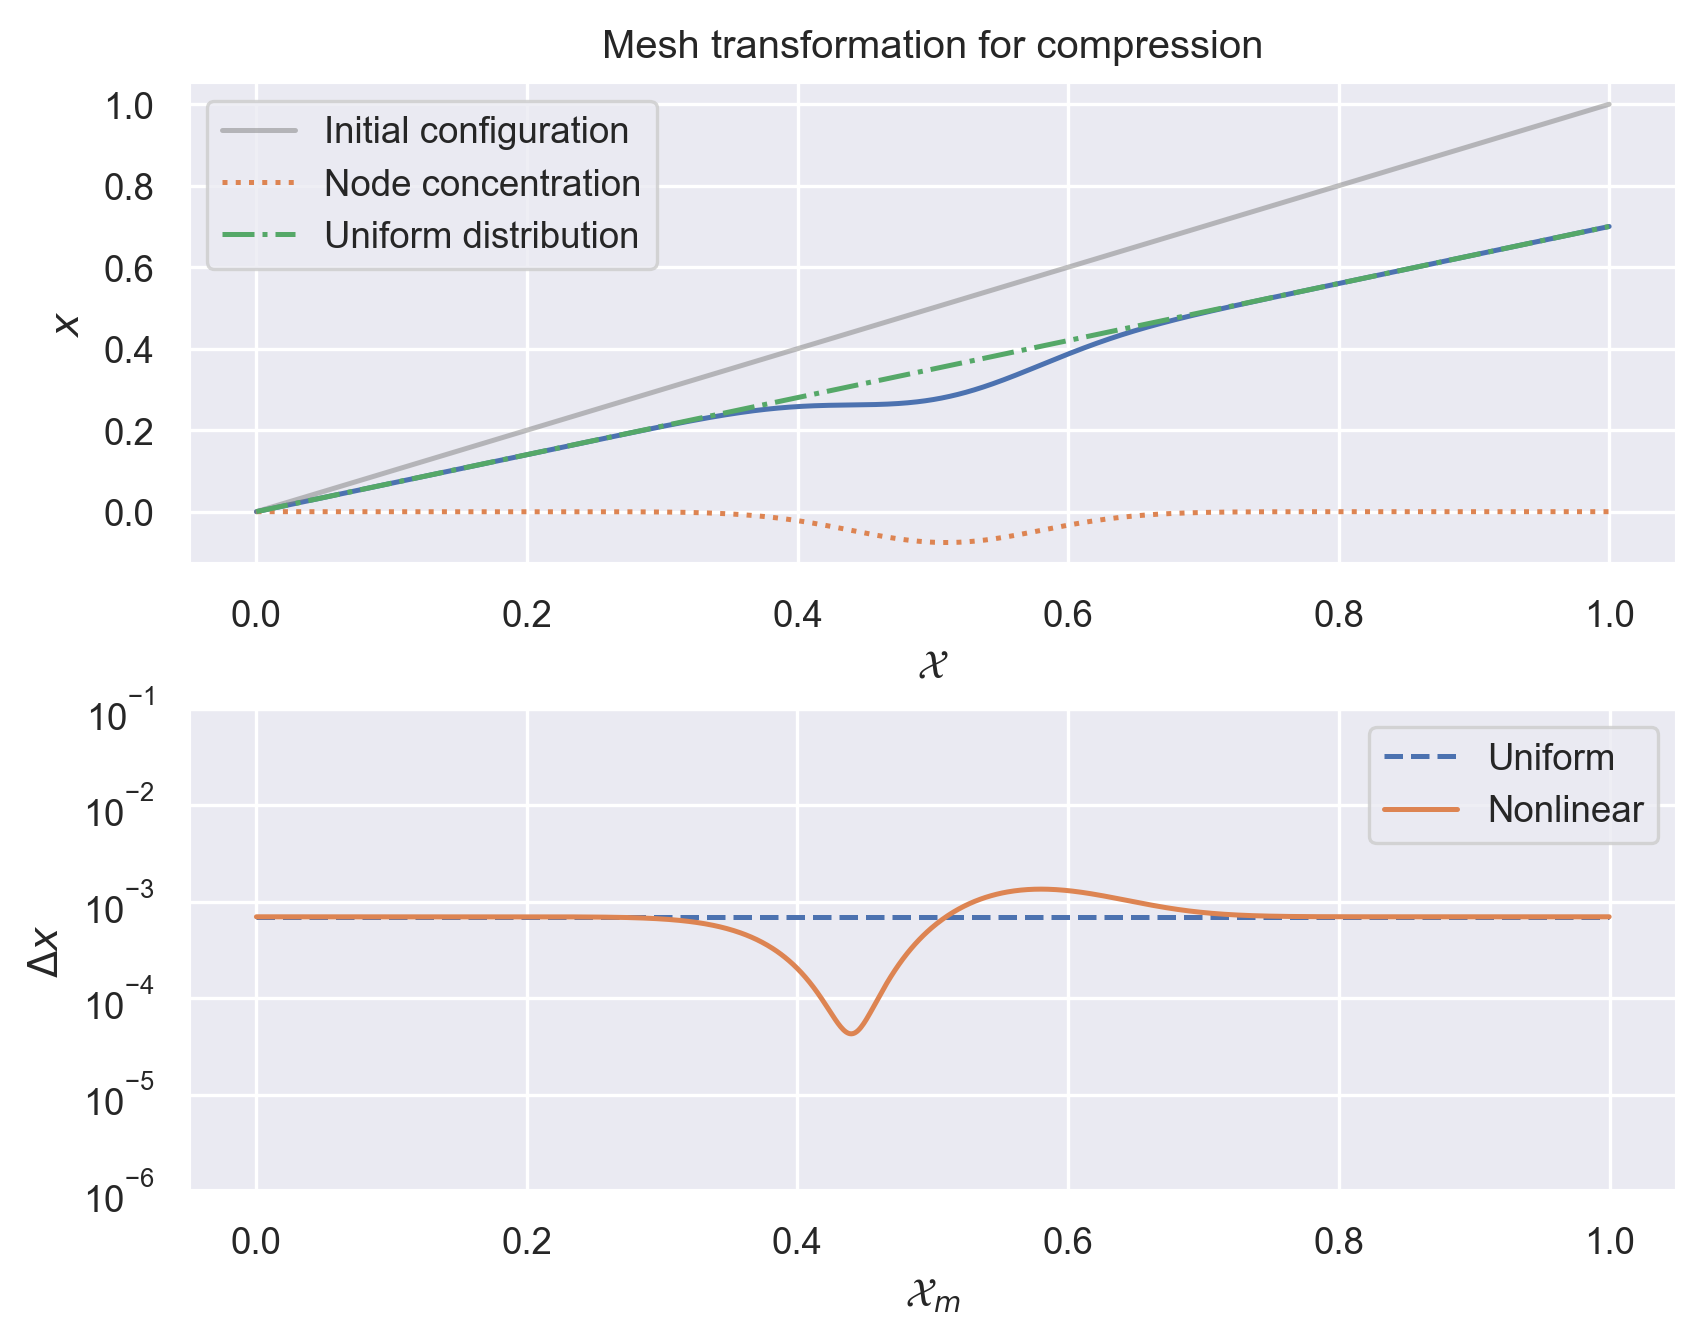
\includegraphics[width =\columnwidth]{research_project/piston/figures/nonlinear_displacement/separable/mapping_mu_05_sigma_01_p_05_compression.png}
    \caption{Feasible mesh compression. 
    The green line shows the maximum piston compression.
    The nodes are locally compressed to the left of the Gaussian curve.}
    \label{fig:mesh_disp_compression}
\end{figure}
\begin{figure}[h]
    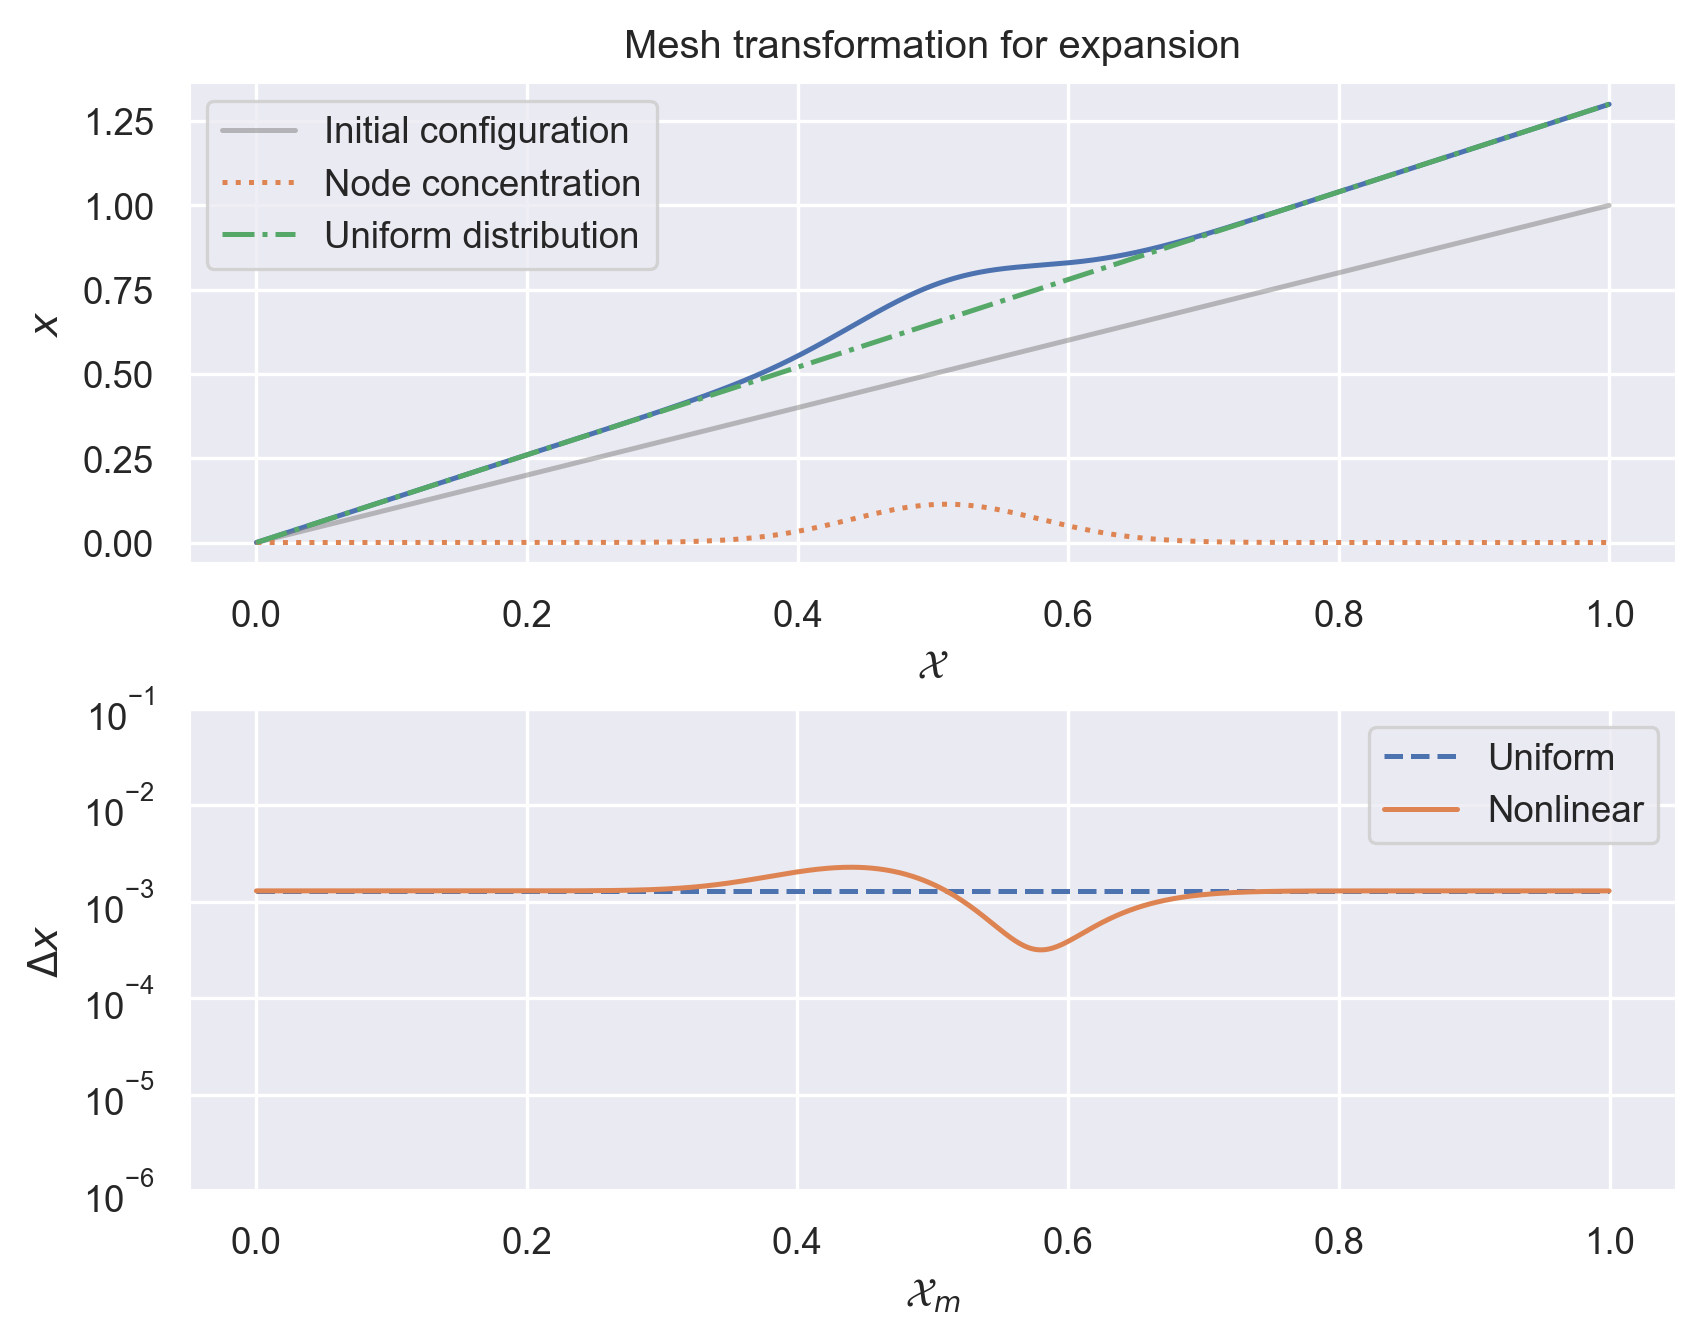
\includegraphics[width =\columnwidth]{research_project/piston/figures/nonlinear_displacement/separable/mapping_mu_05_sigma_01_p_075_expansion.png}
    \caption{Feasible mesh expansion. 
    The green line shows the maximum piston expansion.
    The nodes are locally compressed to the right of the Gaussian curve.}
    \label{fig:mesh_disp_expansion}
\end{figure}

\newpage
\begin{figure}[h]
    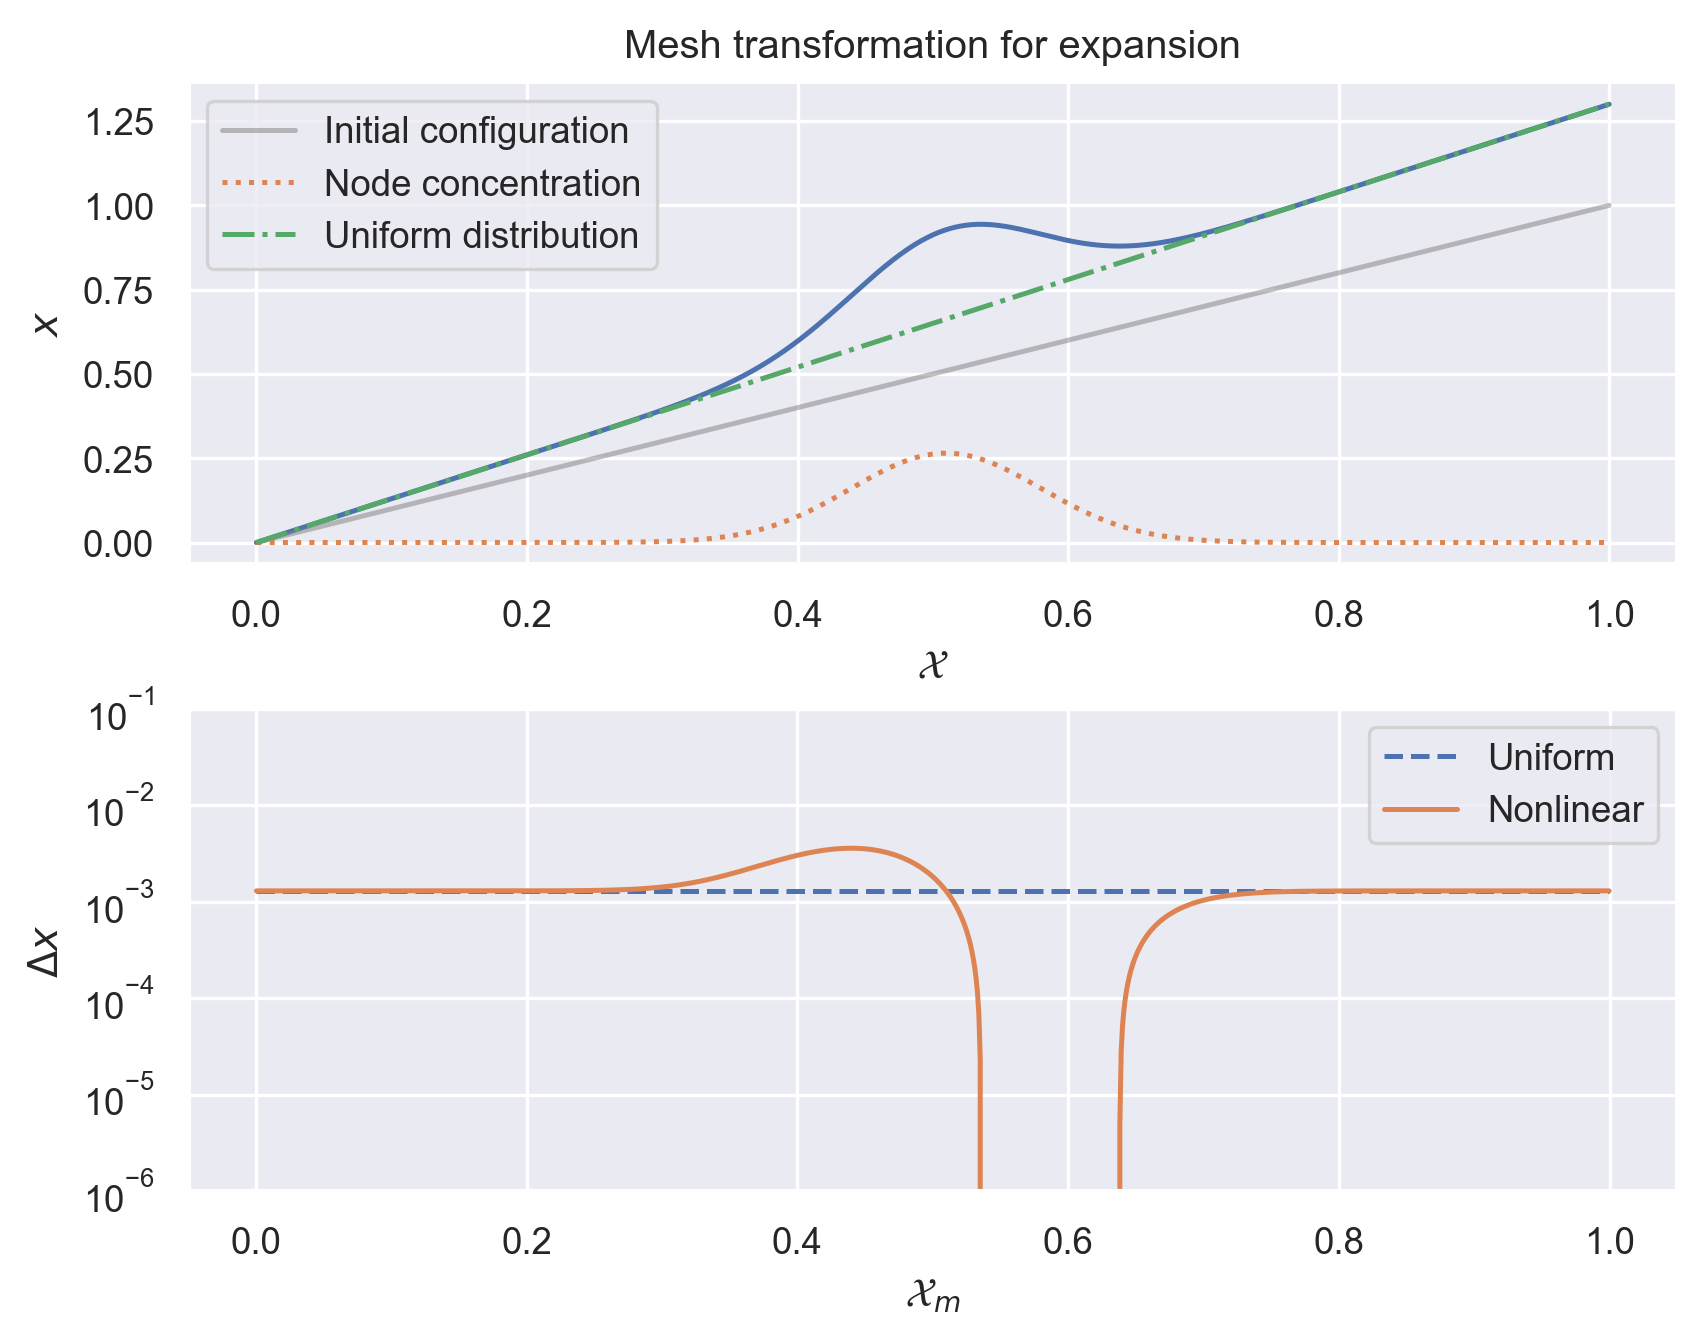
\includegraphics[width =\columnwidth]{research_project/piston/figures/nonlinear_displacement/separable/mapping_mu_05_sigma_01_p_175_expansion.png}
    \caption{Unfeasible mesh expansion.
    Due to the large mesh distortion, the ordering is lost in the physical domain,
    leading to negative mesh step sizes.}
    \label{fig:mesh_disp_expansion_unfeasible}
\end{figure}

\newpage
\subsection{Geometric Conservation Law}
As mentioned in the literature review regarding deforming meshes, 
in Section \ref{sec:literature_review_deforming_mesh},
a proxy to determine how affected is a discretization by a moving mesh
is to attempt the resolution of the constant solution.

This is so because if the discretization is not handling the movement of the mesh correctly,
artificial fluxes of information might be introduced. 
Nevertheless, no strict conclusions can be reached with this numerical test.
Succesfully integrating the constant solution seems 
to be a sufficient but not a necessary condition for stability.

Our implementation seems unable to reproduce correctly the constant solution.
This happens in a fixed and moving mesh setting (see Figure~\ref{fig:ale_effect_constant_solution}).
Therefore, we believe it could be due to the accumulation of round-off errors, 
as previous works have reported in the literature \cite{liu2019balancing}.

In a way, we are surprised that this blowing-up effect does not show up in the piston problem.
We hint towards the fact that, in that context, the constantly changing boundary conditions
somehow lead to balanced round-off errors, which cancel out in time.
In the constant solution test, the boundary condition is constant,
thus potentially preventing round-off error cancellation.

Chasing to the detail this behaviour is certainly meaningful, 
but since our reference solution (the piston) does not suffer from these effects,
we limit ourselves to report this behaviour and skip any further investigation, 
as we believe it falls out of the scope of this work. 

\begin{figure}[h]
    \centering
    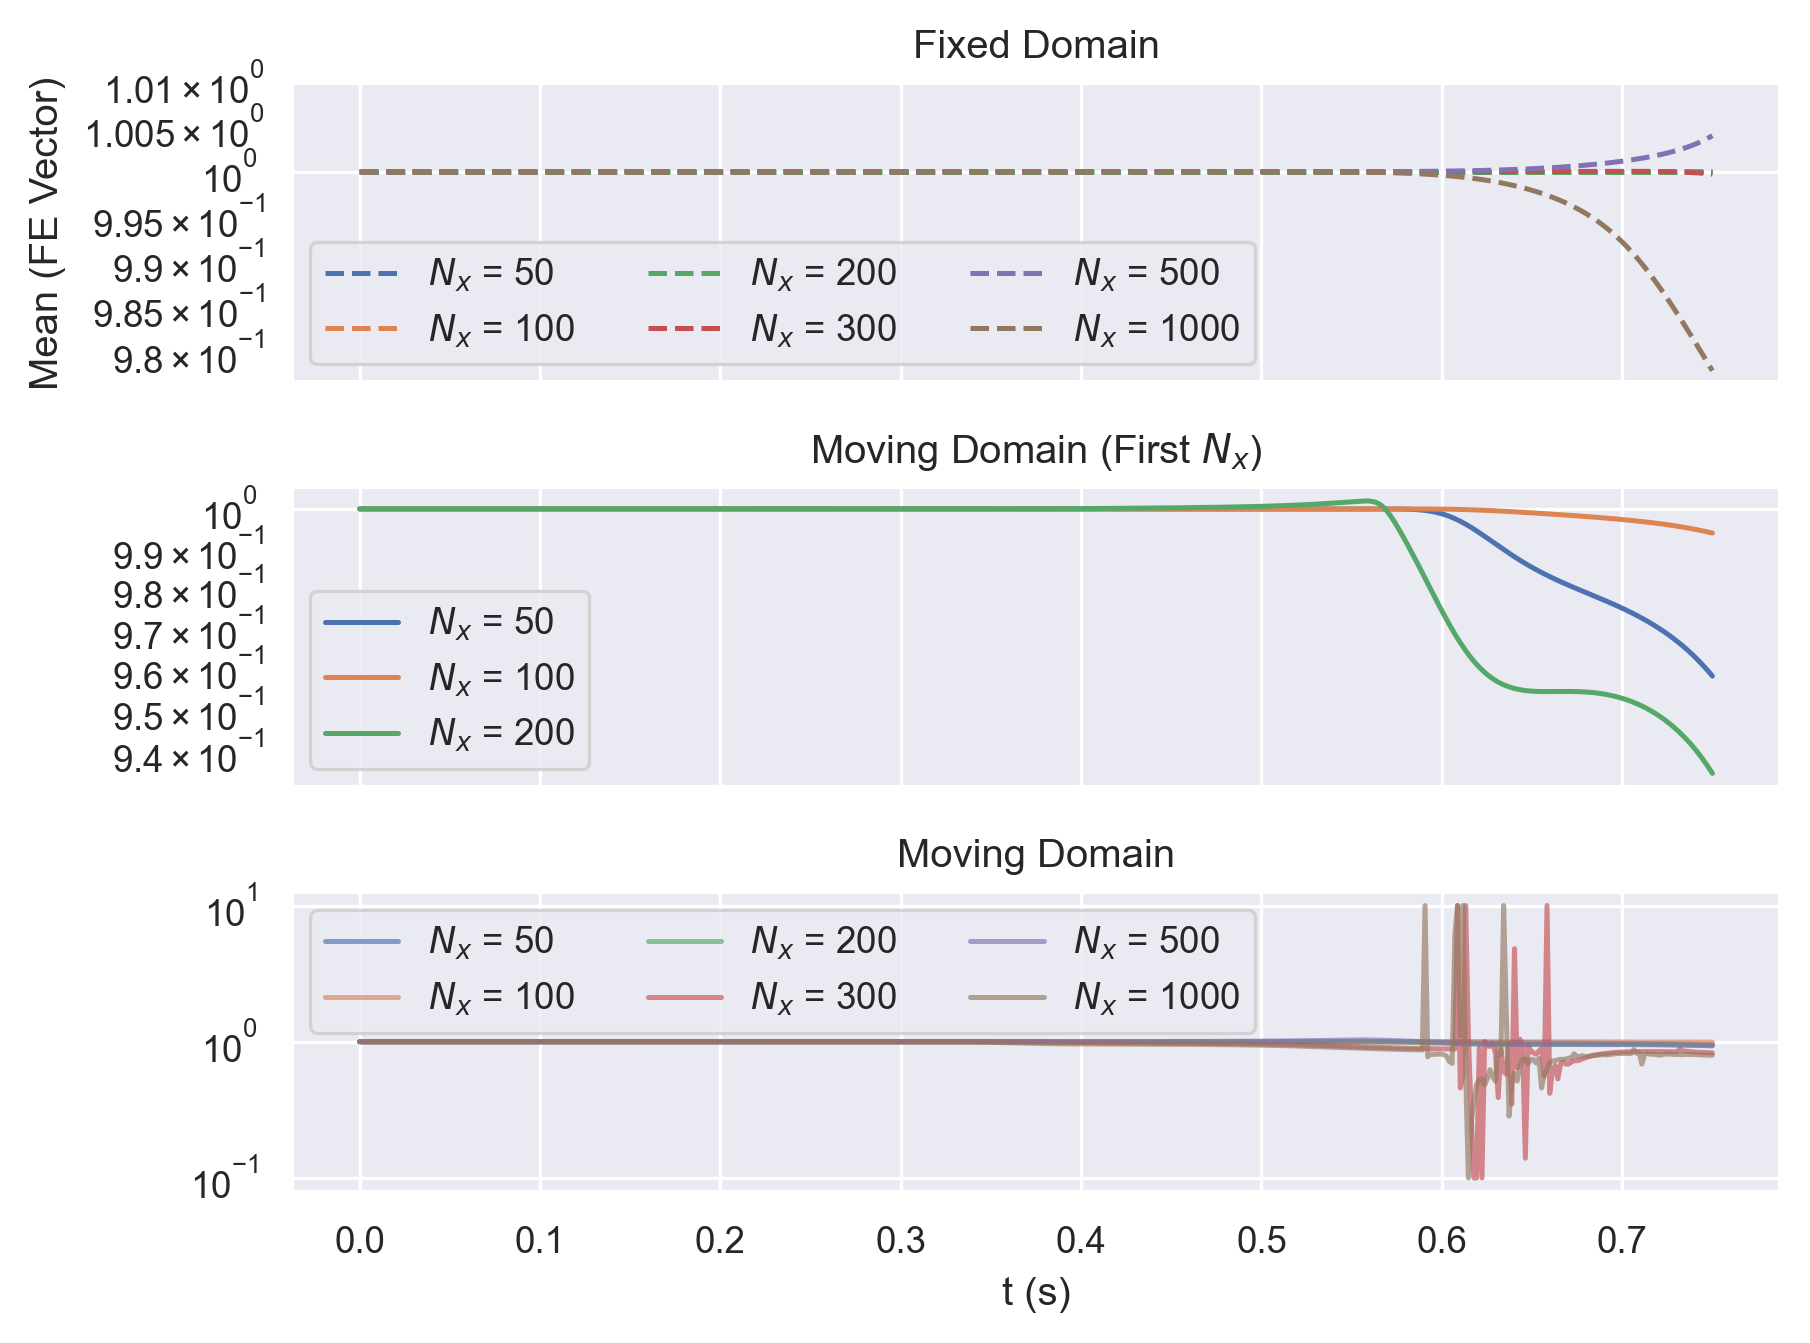
\includegraphics[width=1\columnwidth]{research_project/piston/figures/ale_effect/mean_fe_comparison_constant_solution.png}
    \caption{Constant solution simulation for fixed (top) and moving mesh (middle, bottom).
    The round-off error increases as the number of DoFs increases too ($N_x$). 
    The errors in the fixed mesh take more to accumulate or do not accumulate at all.
    For the moving mesh, for the smallest number of DoFs the solution drifts away from the constant solution.
    In the bottom plot, the values have been clipped to the $[0.01, 10]$ interval.}
    \label{fig:ale_effect_constant_solution}
\end{figure}

\end{document}